\documentclass[11pt,a4paper]{article}

\usepackage[margin=2.5cm]{geometry}
\usepackage{amsmath,amssymb,amsthm,mathtools}
\usepackage{bm}
\usepackage{siunitx}
\usepackage{tikz}
\usetikzlibrary{arrows.meta,positioning}

\title{From Continuous-Time Control to Microcontroller Implementation:\\
	A Professional, Math-Solid Workflow}
\author{Ramon Armeria (portfolio notes)}
\date{\today}

\begin{document}
	\maketitle
	
	\section*{Purpose}
	Provide a rigorous pipeline to implement a feedback controller on a microcontroller while staying mathematically sound: specifications $\to$ plant model $\to$ sampling/holds $\to$ discrete-time design $\to$ implementable difference equations with non-idealities $\to$ verification.
	
	\section{Specifications (What ``Good'' Means)}
	Define performance and robustness before design.
	\begin{itemize}
		\item Performance: rise/settling time, percent overshoot, steady-state error, tracking bandwidth.
		\item Robustness: gain/phase margins, sensitivity peaks, disturbance/noise rejection.
		\item Constraints: actuator saturation and slew limits, word-length/quantization, CPU budget and jitter bounds.
	\end{itemize}
	
	\section{Continuous Plant Modeling}
	Prefer state space; include delays if present.
	\begin{align*}
		\dot x(t) &= A x(t) + B u(t), \qquad y(t) = C x(t) + D u(t),\\
		G(s) &= C (sI - A)^{-1} B + D.
	\end{align*}
	If only a transfer function is available, ensure it is proper, note unstable/non-minimum-phase zeros, and model pure delays (e.g.\ $e^{-s\tau}$).
	
	\section{Sampling, ADC/DAC, and Holds}
	Insert the microcontroller as a sampled-data element.
	\begin{itemize}
		\item Sampling: $x[k] \coloneqq x(kT_s)$ with sampling period $T_s$.
		\item Zero-order hold (ZOH) on DAC: $u(t) = u[k]$ for $t\in[kT_s,(k{+}1)T_s)$.
		\item Anti-alias analog prefilter with cutoff $\approx 0.3\text{--}0.4\,f_s$.
		\item Rule of thumb: $f_s \ge 20\text{--}30\times$ target closed-loop bandwidth.
	\end{itemize}
	
	\section{Discretization (Exact State-Space Preferred)}
	Given $T_s$,
	\begin{align*}
		A_d &= e^{A T_s},\qquad
		B_d = \int_0^{T_s} e^{A\tau}\,d\tau\,B,\qquad
		C_d = C,\quad D_d = D.
	\end{align*}
	Then the sampled plant is
	$$
	x[k{+}1] = A_d x[k] + B_d u[k], \qquad y[k] = C_d x[k] + D_d u[k].
	$$
	Alternative controller discretizations (if you designed $C(s)$):
	\begin{itemize}
		\item \emph{Tustin (bilinear)}: $s \mapsto \dfrac{2}{T_s}\dfrac{z-1}{z+1}$ (optionally prewarp at crossover).
		\item \emph{Matched pole--zero}: map $s$-poles/zeros via $z = e^{sT_s}$.
		\item \emph{Forward/Backward Euler}: quick but more phase/steady-state bias.
	\end{itemize}
	
	\section{Digital Controller Forms and Implementation}
	Express the controller as a $z$-transfer or explicit difference equation.
	\[
	u[k] = \sum_{i=1}^{n_a} \alpha_i\,u[k-i] + \sum_{j=0}^{n_b} \beta_j\,e[k-j],
	\]
	or in controller state-space:
	\[
	x_c[k{+}1] = A_c x_c[k] + B_c e[k],\qquad u[k] = C_c x_c[k] + D_c e[k].
	\]
	Implementation notes:
	\begin{itemize}
		\item Use numerically robust structures (e.g.\ Direct Form II Transposed).
		\item Include one-sample computational delay in validation models.
		\item Ensure bumpless transfer when enabling/disabling control.
	\end{itemize}
	
	\section{Non-Idealities (Professional-Grade Details)}
	\paragraph{Actuator saturation and anti-windup.} Back-calculation (continuous) and its discrete counterpart:
	$$
	\dot x_I = e(t) + k_{aw}\big(u_{\text{sat}} - u\big)
	\quad\leadsto\quad
	x_I[k] = x_I[k{-}1] + T_s\,e[k] + k_{aw} T_s \big(u_{\text{sat}}[k{-}1]-u[k{-}1]\big).
	$$
	
	\paragraph{Rate limits.} Limit $\Delta u$ per sample to reflect actuator slew.
	
	\paragraph{Quantization/word-length.} Model ADC/DAC quantization and finite precision; check for limit cycles.
	
	\paragraph{Timing/jitter.} Guarantee worst-case execution $\le 20\%$ of $T_s$; bound ISR jitter and validate its effect on phase margin.
	
	\paragraph{Noise shaping.} Filter derivative paths; avoid differentiating noise; consider setpoint weighting.
	
	\section{Worked Example: PI $\to$ Discrete (Tustin) with Anti-Windup}
	Continuous PI:
	$$
	C(s) = K_p + \frac{K_i}{s}.
	$$
	Tustin mapping $s \mapsto \dfrac{2}{T_s}\dfrac{z-1}{z+1}$ yields
	$$
	C(z) = K_p + K_i \frac{T_s}{2}\cdot \frac{z+1}{z-1}.
	$$
	A practical realization (trapezoidal integration + back-calculation anti-windup):
	\[
	\begin{aligned}
		e[k]   &= r[k] - y[k],\\
		x_I[k] &= x_I[k-1] + \frac{T_s K_i}{2}\big(e[k] + e[k-1]\big)
		+ k_{aw}\big(u_{\text{sat}}[k-1] - u[k-1]\big),\\
		u^{\ast}(k) &= K_p\,e[k] + x_I[k],\\
		u[k] &= \operatorname{sat}\big(u^{\ast}(k)\big).
	\end{aligned}
	\]
	
	Notes:
	\begin{itemize}
		\item If later adding a $D$ term, use a first-order low-pass on the measured derivative.
		\item Validate with ZOH + one-sample delay in the loop model.
	\end{itemize}
	
	\section{Verification: MIL $\to$ SIL $\to$ HIL $\to$ Bench}
	\begin{enumerate}
		\item \textbf{MIL} (Model-in-the-Loop): simulate plant + ZOH + delay + noise + quantization.
		\item \textbf{SIL} (Software-in-the-Loop): run the real controller code against the simulator.
		\item \textbf{HIL}: place the microcontroller in loop with a real-time plant model.
		\item \textbf{Bench}: low-risk region first; steps, sine sweeps; margins and saturation logs.
	\end{enumerate}
	
	\section{Block Diagram (Sampled-Data View)}
	\begin{center}
		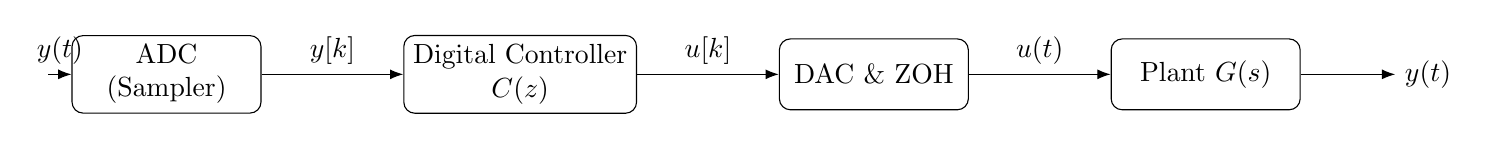
\begin{tikzpicture}[>=Latex, node distance=1.6cm]
			\tikzstyle{blk}=[draw, rounded corners, minimum width=2.4cm, minimum height=0.9cm, align=center]
			\node[blk] (sampler) {ADC\\(Sampler)};
			\node[blk, right=1.8cm of sampler] (ctrl) {Digital Controller\\$C(z)$};
			\node[blk, right=1.8cm of ctrl] (zoh) {DAC \& ZOH};
			\node[blk, right=1.8cm of zoh] (plant) {Plant $G(s)$};
			\draw[->] (-1.5,0) -- (sampler.west) node[midway, above] {$y(t)$};
			\draw[->] (sampler.east) -- (ctrl.west) node[midway, above] {$y[k]$};
			\draw[->] (ctrl.east) -- (zoh.west) node[midway, above] {$u[k]$};
			\draw[->] (zoh.east) -- (plant.west) node[midway, above] {$u(t)$};
			\draw[->] (plant.east) -- ++(1.2,0) node[right] {$y(t)$};
		\end{tikzpicture}
	\end{center}
	
	\section{Rules of Thumb (Quick Checklist)}
	\begin{itemize}
		\item $f_s \ge 20\text{--}30\times$ desired closed-loop bandwidth; anti-alias filter at $0.3\text{--}0.4\,f_s$.
		\item Include ZOH and one-sample computational delay in loop analysis.
		\item Keep CPU load $< 20\%$ of $T_s$; bound jitter; log saturation and overflows.
		\item Use anti-windup where saturation is possible; verify with disturbances and setpoint steps.
	\end{itemize}
	
	\section{Mathematical Concepts You Will Need}
	\subsection*{Foundations}
	\begin{itemize}
		\item Linear ODEs; existence/uniqueness; solutions via matrix exponentials.
		\item Linear Time-Invariant (LTI) systems; convolution; impulse and step responses.
		\item Laplace transform; transfer functions; poles/zeros; BIBO stability.
		\item Frequency response; Bode and Nyquist plots; margins; sensitivity functions.
	\end{itemize}
	
	\subsection*{Sampled-Data and Discrete-Time}
	\begin{itemize}
		\item Sampling theory (Shannon--Nyquist), aliasing, anti-alias filtering.
		\item $z$-transform; regions of convergence; mapping $z=e^{sT_s}$; unit circle stability.
		\item Zero-order hold (ZOH) and step-invariant (hold-equivalent) discretization.
		\item Discretization methods: Forward/Backward Euler, Tustin (bilinear) with prewarping, matched pole--zero.
		\item Discrete-time state space: $A_d=e^{AT_s}$, $B_d=\int_0^{T_s} e^{A\tau}B\,d\tau$; exact discretization.
		\item Difference equations; canonical implementation forms (Direct I/II, transposed).
		\item Discrete-time stability tests: Jury criterion; Schur stability; discrete Lyapunov equation
		$$
		A_d^\top P A_d - P = -Q,\quad Q\succ 0 \Rightarrow P\succ 0.
		$$
	\end{itemize}
	
	\subsection*{Modern Design (Optional but Powerful)}
	\begin{itemize}
		\item Controllability/observability; pole placement.
		\item LQR/LQG; Riccati equations; Kalman filtering; covariance propagation.
		\item Disturbance models, white noise, and power spectral densities.
		\item Internal Model Principle (for zero steady-state error to classes of inputs).
	\end{itemize}
	
	\subsection*{Implementation and Non-Idealities}
	\begin{itemize}
		\item Quantization models (uniform, saturation); fixed- vs floating-point; roundoff/overflow; limit cycles.
		\item Computational delay and jitter modeling in discrete time.
		\item Saturation, anti-windup schemes (back-calculation, conditional integration).
		\item Rate limiting; actuator dynamics; PWM as effective DAC (averaging models).
	\end{itemize}
	
	\subsection*{Validation and Robustness}
	\begin{itemize}
		\item Sensitivity and complementary sensitivity: $S=(I+GC)^{-1}$, $T=GC(I+GC)^{-1}$.
		\item Uncertainty models (gain/phase, additive/multiplicative); margin interpretation in sampled systems.
		\item Monte Carlo and worst-case analyses (parameter spreads, quantization, noise).
	\end{itemize}
	\section{Suggested Literature (with Mathematical Emphasis)}
	
	To develop a solid and professional mathematical foundation for digital control implementation, the following references are recommended. Each entry lists the most relevant chapters or sections for the topics in Section~7.
	
	\subsection*{Classical Control Foundations}
	\begin{itemize}
		\item K. Ogata, \emph{Modern Control Engineering}, 5th ed. (Prentice Hall, 2010).  
		\begin{itemize}
			\item Ch.~2: Mathematical models of systems (ODEs, transfer functions).  
			\item Ch.~3: State-space representation.  
			\item Ch.~4--6: Time response, stability, and root locus.  
			\item Ch.~8: Frequency response methods.  
		\end{itemize}
		\item N.~S. Nise, \emph{Control Systems Engineering}, 7th ed. (Wiley, 2015).  
		\begin{itemize}
			\item Ch.~2--3: Mathematical models of mechanical/electrical systems.  
			\item Ch.~5: Transient response, steady-state error.  
			\item Ch.~10: PID controllers and tuning.  
		\end{itemize}
	\end{itemize}
	
	\subsection*{Signals and Transforms}
	\begin{itemize}
		\item A.~V. Oppenheim and A.~S. Willsky, \emph{Signals and Systems}, 2nd ed. (Pearson, 1997).  
		\begin{itemize}
			\item Ch.~2: Linear time-invariant systems, convolution.  
			\item Ch.~3: Fourier representation, frequency response.  
			\item Ch.~4: Laplace transform.  
			\item Ch.~10: Sampling theorem and reconstruction.  
		\end{itemize}
		\item A.~Oppenheim and R.~Schafer, \emph{Discrete-Time Signal Processing}, 3rd ed. (Pearson, 2009).  
		\begin{itemize}
			\item Ch.~3: $z$-transform.  
			\item Ch.~4: Discrete-time systems and difference equations.  
			\item Ch.~7: Discrete Fourier Transform and FFT.  
			\item Ch.~10: Sampling and multirate systems.  
		\end{itemize}
	\end{itemize}
	
	\subsection*{Digital and Sampled-Data Control}
	\begin{itemize}
		\item G.~F. Franklin, J.~D. Powell, and M.~Workman, \emph{Digital Control of Dynamic Systems}, 3rd ed. (Addison Wesley, 1998).  
		\begin{itemize}
			\item Ch.~3: Sampling and data reconstruction (ADC, DAC, ZOH).  
			\item Ch.~4: $z$-transform methods.  
			\item Ch.~5: Discrete-time system analysis.  
			\item Ch.~6: Discrete controller design (root locus, frequency domain).  
			\item Ch.~7: State-space methods for discrete-time systems.  
		\end{itemize}
		\item K. Åström and B. Wittenmark, \emph{Computer-Controlled Systems: Theory and Design}, 3rd ed. (Prentice Hall, 1997).  
		\begin{itemize}
			\item Ch.~2: Sampled-data models.  
			\item Ch.~3: Discrete-time models.  
			\item Ch.~5: Design in the frequency domain.  
			\item Ch.~7: State feedback and observers in discrete time.  
			\item Ch.~9: Implementation issues (quantization, timing).  
		\end{itemize}
	\end{itemize}
	
	\subsection*{Modern Control and Robustness}
	\begin{itemize}
		\item T. Kailath, \emph{Linear Systems} (Prentice Hall, 1980).  
		\begin{itemize}
			\item Ch.~1--2: Linear spaces, operators, and system descriptions.  
			\item Ch.~3: Controllability, observability.  
			\item Ch.~5: Stability and Lyapunov methods.  
		\end{itemize}
		\item B. Anderson and J. Moore, \emph{Optimal Control: Linear Quadratic Methods} (Prentice Hall, 1990).  
		\begin{itemize}
			\item Ch.~2: Discrete-time Riccati equations.  
			\item Ch.~3--4: LQR design in discrete time.  
		\end{itemize}
		\item S. Skogestad and I. Postlethwaite, \emph{Multivariable Feedback Control: Analysis and Design}, 2nd ed. (Wiley, 2005).  
		\begin{itemize}
			\item Ch.~2: Sensitivity functions, robustness concepts.  
			\item Ch.~6--7: Frequency-domain design methods.  
			\item Ch.~11: Uncertainty modeling and robust stability.  
		\end{itemize}
	\end{itemize}
	
	\subsection*{Numerical and Implementation Aspects}
	\begin{itemize}
		\item G.~H. Golub and C.~F. Van Loan, \emph{Matrix Computations}, 4th ed. (Johns Hopkins, 2013).  
		\begin{itemize}
			\item Ch.~9: Matrix exponentials (for exact discretization).  
			\item Ch.~10--11: Numerical stability of algorithms.  
		\end{itemize}
		\item B. Widrow and I. Kollár, \emph{Quantization Noise} (Cambridge University Press, 2008).  
		\begin{itemize}
			\item Ch.~1--3: Models of quantization.  
			\item Ch.~6: Quantization in feedback systems.  
		\end{itemize}
	\end{itemize}
	\section*{Bio-Pump Aquarium Controller: Modeling, Control, and Roadmap}
	
	\subsection*{System Overview}
	\textbf{Plant:} water tank with pump (flow), heater (temperature), aeration (DO), dosing (acid/base, buffer).\\
	\textbf{Sensors:} temperature, turbidity, pH, electrical conductivity (EC), dissolved oxygen (DO), optional ORP.\\
	\textbf{Actuators:} PWM pump, SSR/relay heater, aeration pump/valve, peristaltic dosing pumps.\\
	\textbf{Controller:} microcontroller (ESP32/STM32), isolated analog front-end, logging.
	
	\subsection*{Complexity Tiers}
	\begin{itemize}
		\item \textbf{Tier A (MVP):} Temperature PID; flow PI; turbidity alarm; logging and basic failsafes.
		\item \textbf{Tier B (Smart):} Add pH, EC, DO sensing; closed-loop pH (conservative PI); DO control; calibration flows; temperature compensation.
		\item \textbf{Tier C (Advanced):} Nitrogen-cycle observer (ammonia/nitrite/nitrate); optional colorimetric nitrate; supervisory MPC; fault diagnosis.
	\end{itemize}
	
	\subsection*{Control Decomposition (SISO Loops + Slow Supervisor)}
	\paragraph{Temperature Loop (Heater)}
	First-order plus delay model (about an operating point):
	$$
	\frac{T(s)}{Q_{\text{heater}}(s)} \approx \frac{K}{\tau s + 1}\,e^{-Ls}.
	$$
	Discrete PID (Tustin), with back-calculation anti-windup:
	$$
	\begin{aligned}
		e[k]   &= T_{\text{set}} - T[k],\\
		x_I[k] &= x_I[k{-}1] + \frac{T_s K_i}{2}\big(e[k] + e[k{-}1]\big) + k_{aw}\big(u_{\text{sat}}[k{-}1] - u[k{-}1]\big),\\
		u^{*} \big[k] &= K_p\,e[k] + x_I[k] + K_d\,\frac{2}{T_s}\big(T[k{-}1] - T[k]\big),\\
		u[k] &= \operatorname{sat}\!\big(u^{*}\big [k]\big).
	\end{aligned}
	$$
	
	\paragraph{Flow Loop (Pump)}
	Local linearization around nominal PWM $\to$ PI control on measured/estimated flow $q$:
	$$
	e_q[k] = q_{\text{set}} - q[k],\qquad u_q[k] = K_{p,q}\,e_q[k] + x_{I,q}[k],
	$$
	with the same integral update/anti-windup structure as above.
	
	\paragraph{pH Loop (Dosing)}
	Integrating and delayed plant $\Rightarrow$ conservative PI, minimum dose quanta $\Delta u_{\min}$ and lockout:
	$$
	\begin{aligned}
		e_{\text{pH}}[k] &= \text{pH}_{\text{set}} - \text{pH}[k],\\
		x_{I,\text{pH}}[k] &= x_{I,\text{pH}}[k{-}1] + T_s K_{i,\text{pH}}\,e_{\text{pH}}[k],\\
		u_{\text{dose}}[k] &= \mathcal{Q}_{\Delta u_{\min}}\!\left(\operatorname{sat}_{[0,u_{\max}]}\big(K_{p,\text{pH}}e_{\text{pH}}[k] + x_{I,\text{pH}}[k]\big)\right),
	\end{aligned}
	$$
	with daily caps and time lockouts to prevent overshoot.
	
	\paragraph{DO Loop (Aeration)}
	First-order oxygenation dynamics $\Rightarrow$ PI on DO:
	$$
	e_{\text{DO}}[k] = \text{DO}_{\text{set}} - \text{DO}[k],\qquad u_{\text{air}}[k] = K_{p,\text{DO}}\,e_{\text{DO}}[k] + x_{I,\text{DO}}[k].
	$$
	
	\paragraph{Supervisory Layer (Slow)}
	Schedules feeding/backwash, freezes pH dosing during disturbances, adjusts setpoints (e.g.\ higher DO post-feeding), enforces interlocks and dose caps.
	
	\subsection*{Nitrogen Cycle (Minimal State Model)}
	Let $N_{\mathrm{H3}}$, $N_{\mathrm{NO_2}}$, $N_{\mathrm{NO_3}}$ be ammonia, nitrite, nitrate concentrations. With effective biomasses $X_{\mathrm{AOB}},X_{\mathrm{NOB}},X_{\mathrm{DEN}}$ and Arrhenius-type rates $k_i(T)$:
	$$
	\begin{aligned}
		\dot N_{\mathrm{H3}}   &= I_{\text{feed}} - k_1(T)\,X_{\mathrm{AOB}}\,N_{\mathrm{H3}},\\
		\dot N_{\mathrm{NO_2}} &= k_1(T)\,X_{\mathrm{AOB}}\,N_{\mathrm{H3}} - k_2(T)\,X_{\mathrm{NOB}}\,N_{\mathrm{NO_2}},\\
		\dot N_{\mathrm{NO_3}} &= k_2(T)\,X_{\mathrm{NOB}}\,N_{\mathrm{NO_2}} - k_3(T)\,X_{\mathrm{DEN}}\,N_{\mathrm{NO_3}}.
	\end{aligned}
	$$
	These ODEs serve as an observer backbone; occasional manual/colorimetric nitrate measurements re-anchor the state.
	
	\subsection*{Sensor Compensation and Filtering}
	Temperature compensation (example affine models around $25^\circ$C):
	$$
	\text{pH}_{25} \approx \text{pH}_T + \alpha\,(T-25^\circ\mathrm{C}),\qquad
	\kappa_{25} \approx \frac{\kappa_T}{1 + \beta\,(T-25^\circ\mathrm{C})}.
	$$
	Apply median/IIR filtering to reduce noise; respect probe-specific calibration parameters.
	
	\subsection*{Sampling \& Tasking (Typical)}
	\begin{itemize}
		\item Fast (50--200 Hz): pump current/flow proxy and debouncing.
		\item Medium (1--5 Hz): temperature, turbidity, EC.
		\item Slow (0.2--1 Hz): pH, DO, ORP.
	\end{itemize}
	
	\subsection*{Safety Constraints (Illustrative)}
	\begin{itemize}
		\item Heater hard cutoff (thermal fuse) $+$ firmware limit $u \le u_{\max}$.
		\item Dosing quantization $\Delta u_{\min}$, per-interval lockout, daily dose cap.
		\item Sensor sanity bounds and recalibration prompts; watchdog and brown-out reset.
		\item Electrical isolation between noisy motor domain and sensitive analog front-end.
	\end{itemize}
	
	\subsection*{Implementation Roadmap}
	\begin{enumerate}
		\item \textbf{Phase 1:} Temp PID $+$ Flow PI $+$ turbidity alarm; logging/UI.
		\item \textbf{Phase 2:} Add pH/EC sensing; manual guided dosing with compensation.
		\item \textbf{Phase 3:} Closed-loop pH (conservative PI); DO sensing and PI aeration.
		\item \textbf{Phase 4:} Scheduling (feeding/backwash) and safety envelopes.
		\item \textbf{Phase 5:} Nitrate colorimetry $+$ EKF observer; trial MPC.
	\end{enumerate}
	
	\subsection*{Notes on Discretization \& Tuning}
	Use Tustin (bilinear) for PI/PID, zero-order hold for internal linear models. Enforce anti-windup via back-calculation:
	$$
	x_I \gets x_I + k_{aw}\,(u_{\text{sat}}-u),\qquad u = \operatorname{sat}(u^{*}\big).
	$$
	Tune via step tests around operating points; validate with logged data and staged safeties.
	
\end{document}
